\documentclass[a4paper]{llncs}
\usepackage[utf8]{inputenc}
\usepackage[T1]{fontenc}
\usepackage{lmodern}
\usepackage[australian,american]{babel}
\usepackage[backend=biber,style=lncs,bibencoding=utf8,sorting=none]{biblatex}
\usepackage{amsfonts}
\usepackage{csquotes}
\usepackage[usenames, dvipsnames]{xcolor}
\usepackage{tikz}
\usepackage{multirow}
\usepackage{pgfplots}
\usepackage{booktabs}
\usepackage{siunitx}
\usepackage{algorithm2e}
\usepackage[super]{nth}
\usepackage[hidelinks]{hyperref}

\pgfplotsset{compat=1.5}


\bibliography{references}
\pagestyle{plain}
%\nocite{*}

\begin{document}
\title{Tree-Based Routing}

%If you're using runningheads you can add an abreviated title for the running head on odd pages using the following
%\titlerunning{abreviated title goes here}
%and an alternative title for the table of contents:
%\toctitle{table of contents title}

\subtitle{Sensor Networks and Internet of Things}

%For multiple authors:
\author{Sébastien Vaucher \and Benjamin Bediako}


%If using runnningheads you can abbreviate the author name on even pages:
%\authorrunning{abbreviated author name}
%and you can change the author name in the table of contents
%\tocauthor{enhanced author name}

% If authors are from different institutes 
\institute{Université de Neuchâtel\\Neuchâtel, Switzerland\\ \email{\{\href{mailto:sebastien.vaucher@unine.ch}{sebastien.vaucher},\href{mailto:benjamin.bediako@unine.ch}{benjamin.bediako}\}@unine.ch}}

%to remove your email just remove '\email{email address}'
% you can also remove the thanks footnote by removing '\thanks{Thank you to...}'


\maketitle
\thispagestyle{plain}
%\begin{abstract}
%abstract text goes here - Lorem ipsum dolor sit amet, consectetur adipiscing elit, sed do eiusmod tempor incididunt ut labore et dolore magna aliqua.
%\end{abstract}

\section{Introduction}

This report presents the results obtained during the project of the Sensor Networks and Internet of Things lecture taught at the University of Bern.
The goal of the project is to implement a tree-based routing protocol on top of the Contiki platform.
The implementation is programmed in the C programming language.

This document is structured as follows.
The first section contains a theoretical introduction of the protocol.
In the second part, the implementation is discussed.
Finally, we evaluate different variants of the protocol and discuss the results.

\section{Protocol Description}

This section describes the routing protocol which we were tasked to implement.

In a wireless sensor network, a number of nodes collaborate to provide sensor data to a more powerful computer for further analysis.
Our deployment considers a single aggregator, commonly called the \textit{sink}.
A number of low-power sensor nodes will sense data at their location and then send values towards the sink.
As it is not realistically feasible to reach the sink from any location, more distant nodes will forward their data to an intermediate node that is then tasked to send the data towards the sink.

The tree-based routing protocol is elegantly simple.
It only requires broadcast and unicast primitives in the sensor node firmware.
Packet routing, however, is only possible in one direction, viz. from individual nodes to the central sink node.

The tree-based routing protocol works in two phases.
First, the discovery phase will shape paths from each leaf node to the root node.
After this phase is completed, each node knows a route towards the sink that it can use to transfer useful sensor data.

\subsection{Discovery Phase}

\begin{algorithm}[htbp]
\SetKwFunction{Sleep}{Sleep}
\SetKwFunction{Broadcast}{Broadcast}
\SetKwData{WaitTime}{WaitTime}
\SetKwData{SequenceEmitted}{SequenceEmitted}
\SetKwData{DiscoveryMessage}{DiscoveryMessage}
\SetKwData{NodeId}{NodeId}
\KwIn{\\\WaitTime: Time to wait between each discovery phase \\
\NodeId: ID of the root node}
\Begin{
$\SequenceEmitted \leftarrow 0$ \;
\While{$\mathcal{T}$}{
\Sleep{\WaitTime} \;
$\SequenceEmitted \leftarrow \SequenceEmitted + 1$ \;
$\DiscoveryMessage.ParentId \leftarrow \NodeId$ \;
$\DiscoveryMessage.HopCount \leftarrow 1$ \;
$\DiscoveryMessage.SequenceNumber \leftarrow \SequenceEmitted$ \;
\Broadcast{\DiscoveryMessage} \;
}}
\caption{Sink node discovery algorithm}
\label{algo:root}
\end{algorithm}



\begin{algorithm}[htbp]
\SetKwFunction{Sleep}{Sleep}
\SetKwFunction{Broadcast}{Broadcast}
\SetKwData{WaitTime}{WaitTime}
\SetKwData{PreviousSequence}{PreviousSequence}
\SetKwData{DiscoveryMessage}{DiscoveryMessage}
\SetKwData{NewParent}{NewParent}
\SetKwData{ShouldForward}{ShouldForward}
\SetKwData{NodeId}{NodeId}
\KwIn{\\\NodeId: ID of the current node \\
\DiscoveryMessage: An incoming discovery packet \\
\PreviousSequence: Most recent sequence number heard}
\KwOut{\\\NewParent: New parent node}
\Begin{
$\ShouldForward \leftarrow \mathcal{F}$ \;
\uIf{\DiscoveryMessage is the \nth{1} message to ever arrive}{
	$\NewParent \leftarrow \DiscoveryMessage.ParentId$ \;
	$\ShouldForward \leftarrow \mathcal{T}$ \;
}
\Else{
	\If{$\DiscoveryMessage.SequenceNumber > \PreviousSequence$}{
		$\ShouldForward \leftarrow \mathcal{T}$ \;
	}
	\If{$\DiscoveryMessage.ParentId$ would be a better parent}{
		$\NewParent \leftarrow \DiscoveryMessage.ParentId$ \;
		$\ShouldForward \leftarrow \mathcal{T}$ \;
	}
}
\If{$\ShouldForward = \mathcal{T}$}{
	$\DiscoveryMessage.HopCount \leftarrow \DiscoveryMessage.HopCount + 1$ \;
	$\DiscoveryMessage.ParentId \leftarrow \NodeId$ \;
	\Broadcast{\DiscoveryMessage} \;
}}
\caption{Sensor node discovery algorithm}
\label{algo:nonroot}
\end{algorithm}

The discovery phase of the algorithm works by \textit{flooding}.
Discovery messages will be exchanged from the sink to distant nodes.
A discovery message contains the following fields:

\begin{itemize}
\item The parent node ID
\item A hop counter
\item A sequence number
\end{itemize}

The parent node ID is the identifier of the node sending a particular packet.
The hop-count value states how many nodes a packet has traversed.
When a packet originates from any node, the hop-count is always 0.
The value is incremented whenever a node forwards a packet.
The sequence number identifies an instance of a packet.
Nodes that forward a packet must never change this value.
The sequence number is incremented by 1 for each new discovery message created by the root node.
Using this information, sensor nodes can identify whether an incoming packet is new.

The root node constitutes what we will call \enquote{level 0} of the tree.
Its operations are described in \autoref{algo:root}.
In short, the root will broadcast a new discovery packet at regular intervals.

When a sensor node that is not the root receives a discovery packet, it proceeds as shown is \autoref{algo:nonroot}.
Basically, a node will compare the information in the discovery packet with the characteristics of its current parent.
If the parent advertised in the packet would be better (smaller hop-count, better signal strength, etc.), the node assigns it as its parent.
Then, if the packet would be of interest to other nodes -- if it is a new packet coming from the root, or if the hop-count is smaller than a previously forwarded packet -- then, the node will broadcast it.
The process is periodical, so broken links in the system will automatically heal when the next discovery iteration happens.

\subsection{Sending Sensor Data}

The role of the discovery phase was to establish a routing tree.
Sending data to the sink is then trivially simple for the sensor nodes.
Once a sensor node knows a parent, it will routinely send sensor data to it.
The parent node will then forward the packet to its own parent until the sink is reached.

\section{Analysis}

In our implementation, we have two configuration options: the MAC protocol and the metric used to qualify if a parent node is \enquote{better} than another.
We compared two MAC protocols: NullMAC and X-MAC \autocite{xmac}; and two metrics: hop-count and RSSI.
The hop-count metric favorises nodes that are topologically closer to the sink.
The RSSI metric favorises the quality of the reception from the parent node.

We ran our algorithm of the TARWIS testbed of the University of Bern, by batches of \SI{30}{\minute}.



\begin{table}
\centering
\begin{tabular}{lllll}
\toprule
& & \multicolumn{2}{c}{Packet delivery rate} \\
\cmidrule{4-5}
MAC & Strategy & Average hop-count & Global & Connected only \\
\midrule
\multirow{2}{*}{NullMAC} & Hop-count & \\
& RSSI & \\
\multirow{2}{*}{X-MAC} & Hop-count & \\
& RSSI & \\
\bottomrule
\end{tabular}
\caption{Comparative table of different configurations}
\label{tab:comp}
\end{table}

\begin{figure}
	\centering
	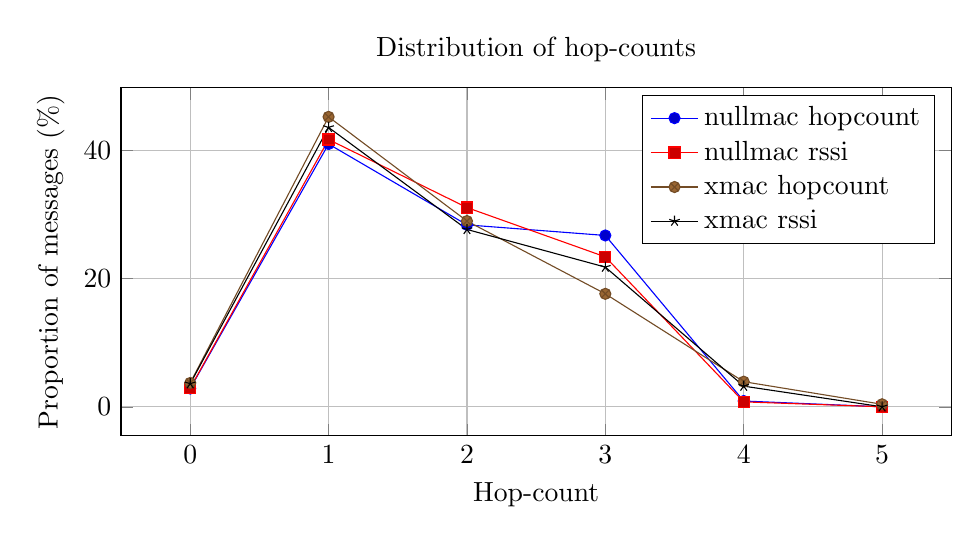
\begin{tikzpicture}
\begin{axis}[
	title=Distribution of hop-counts,
	width=\textwidth,
	height=6cm,
	grid=major,
	ylabel={Proportion of messages (\%)},
	xlabel={Hop-count},
	legend style={
		cells={anchor=west}
	}
]
\addplot coordinates {(0, 2.857142857142857) (1, 41.05263157894737) (2, 28.421052631578947) (3, 26.766917293233083) (4, 0.9022556390977444) (5,0)};
\addplot coordinates {(0, 2.9275808936825885) (1, 41.756548536209553) (2, 31.124807395993837) (3, 23.420647149460708) (4, 0.7704160246533128) (5,0)};
\addplot coordinates {(0, 3.725490196078431) (1, 45.294117647058824) (2, 29.01960784313726) (3, 17.647058823529413) (4, 3.92156862745098) (5, 0.392156862745098)};
\addplot coordinates {(0, 3.6053130929791274) (1, 43.64326375711575) (2, 27.703984819734345) (3, 21.821631878557876) (4, 3.225806451612903) (5,0)};

\legend{nullmac hopcount, nullmac rssi, xmac hopcount, xmac rssi}
\end{axis}
\end{tikzpicture}
	\caption{Distribution of hop-counts with different strategies}
	\label{fig:distribution}
\end{figure}

\begin{figure}
	\centering
	% Generate this file by running the logs/parse_logs.py script
	
    \begin{tikzpicture}[scale=0.097,y= {(0.281cm,0.281cm)}, z={(0cm,1cm)}, x={(1cm,0cm)}]]
    \node[anchor=south west,inner sep=0] at (0,0) {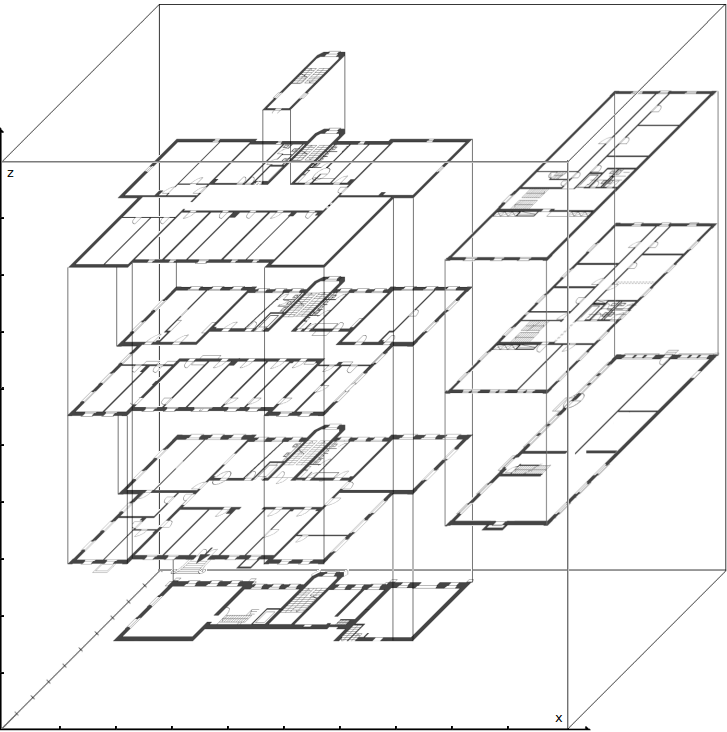
\includegraphics[width=\textwidth]{3D_image_iam_complete.png}};
    \draw [Maroon, thick, dash pattern= on 4mm off 4mm, dash phase=2mm, <-, >=latex] (45,25,52) to (52,30,80);
\draw [Maroon, thick, dash pattern= on 4mm off 4mm, dash phase=2mm, <-, >=latex] (45,25,52) to (45,98,22);
\draw [Maroon, thick, dash pattern= on 4mm off 4mm, dash phase=2mm, <-, >=latex] (45,98,22) to (80,10,80);
\draw [Maroon, thick, dash pattern= on 4mm off 4mm, dash phase=2mm, <-, >=latex] (80,10,80) to (90,100,85);
\draw [Maroon, thick, dash pattern= on 4mm off 4mm, dash phase=2mm, <-, >=latex] (45,25,52) to (53,33,52);
\draw [Maroon, thick, dash pattern= on 4mm off 4mm, dash phase=2mm, <-, >=latex] (45,25,52) to (37,55,52);
\draw [Maroon, thick, dash pattern= on 4mm off 4mm, dash phase=2mm, <-, >=latex] (37,55,52) to (3,75,22);
\draw [Maroon, thick, dash pattern= on 4mm off 4mm, dash phase=2mm, <-, >=latex] (37,55,52) to (20,35,52);
\draw [Maroon, thick, dash pattern= on 4mm off 4mm, dash phase=2mm, <-, >=latex] (45,25,52) to (37,15,80);
\draw [Maroon, thick, dash pattern= on 4mm off 4mm, dash phase=2mm, <-, >=latex] (45,25,52) to (48,65,22);
\draw [Maroon, thick, dash pattern= on 4mm off 4mm, dash phase=2mm, <-, >=latex] (48,65,22) to (90,10,80);
\draw [Maroon, thick, dash pattern= on 4mm off 4mm, dash phase=2mm, <-, >=latex] (48,65,22) to (16,30,22);
\draw [Maroon, thick, dash pattern= on 4mm off 4mm, dash phase=2mm, <-, >=latex] (45,25,52) to (47,85,80);
\draw [Maroon, thick, dash pattern= on 4mm off 4mm, dash phase=2mm, <-, >=latex] (45,25,52) to (45,35,22);
\draw [Maroon, thick, dash pattern= on 4mm off 4mm, dash phase=2mm, <-, >=latex] (45,25,52) to (53,53,80);
\draw [Maroon, thick, dash pattern= on 4mm off 4mm, dash phase=2mm, <-, >=latex] (53,53,80) to (5,60,80);
\draw [Maroon, thick, dash pattern= on 4mm off 4mm, dash phase=2mm, <-, >=latex] (45,25,52) to (19,80,52);
\draw [Maroon, thick, dash pattern= on 4mm off 4mm, dash phase=2mm, <-, >=latex] (19,80,52) to (78,78,57);
\draw [Maroon, thick, dash pattern= on 4mm off 4mm, dash phase=2mm, <-, >=latex] (78,78,57) to (90,100,80);
\draw [Maroon, thick, dash pattern= on 4mm off 4mm, dash phase=2mm, <-, >=latex] (19,80,52) to (18,55,0);
\draw [Maroon, thick, dash pattern= on 4mm off 4mm, dash phase=2mm, <-, >=latex] (19,80,52) to (78,63,57);
\draw [Maroon, thick, dash pattern= on 4mm off 4mm, dash phase=2mm, <-, >=latex] (78,63,57) to (80,75,80);
\draw [Maroon, thick, dash pattern= on 4mm off 4mm, dash phase=2mm, <-, >=latex] (78,63,57) to (93,78,57);
\draw [Maroon, thick, dash pattern= on 4mm off 4mm, dash phase=2mm, <-, >=latex] (45,25,52) to (38,40,22);
\draw [JungleGreen, thick, dash pattern= on 4mm off 4mm, dash phase=6mm, <-, >=latex] (45,25,52) to (38,40,22);
\draw [JungleGreen, thick, dash pattern= on 4mm off 4mm, dash phase=6mm, <-, >=latex] (38,40,22) to (16,30,22);
\draw [JungleGreen, thick, dash pattern= on 4mm off 4mm, dash phase=6mm, <-, >=latex] (16,30,22) to (16,55,22);
\draw [JungleGreen, thick, dash pattern= on 4mm off 4mm, dash phase=6mm, <-, >=latex] (45,25,52) to (37,15,80);
\draw [JungleGreen, thick, dash pattern= on 4mm off 4mm, dash phase=6mm, <-, >=latex] (45,25,52) to (35,20,52);
\draw [JungleGreen, thick, dash pattern= on 4mm off 4mm, dash phase=6mm, <-, >=latex] (45,25,52) to (48,65,22);
\draw [JungleGreen, thick, dash pattern= on 4mm off 4mm, dash phase=6mm, <-, >=latex] (45,25,52) to (45,90,52);
\draw [JungleGreen, thick, dash pattern= on 4mm off 4mm, dash phase=6mm, <-, >=latex] (45,90,52) to (85,33,57);
\draw [JungleGreen, thick, dash pattern= on 4mm off 4mm, dash phase=6mm, <-, >=latex] (85,33,57) to (92,33,57);
\draw [JungleGreen, thick, dash pattern= on 4mm off 4mm, dash phase=6mm, <-, >=latex] (85,33,57) to (78,78,57);
\draw [JungleGreen, thick, dash pattern= on 4mm off 4mm, dash phase=6mm, <-, >=latex] (78,78,57) to (90,100,80);
\draw [JungleGreen, thick, dash pattern= on 4mm off 4mm, dash phase=6mm, <-, >=latex] (45,25,52) to (53,53,80);
\draw [JungleGreen, thick, dash pattern= on 4mm off 4mm, dash phase=6mm, <-, >=latex] (53,53,80) to (80,10,80);
\draw [JungleGreen, thick, dash pattern= on 4mm off 4mm, dash phase=6mm, <-, >=latex] (80,10,80) to (90,100,85);
\draw [JungleGreen, thick, dash pattern= on 4mm off 4mm, dash phase=6mm, <-, >=latex] (45,25,52) to (20,39,80);
\draw [JungleGreen, thick, dash pattern= on 4mm off 4mm, dash phase=6mm, <-, >=latex] (20,39,80) to (20,35,52);
\draw [JungleGreen, thick, dash pattern= on 4mm off 4mm, dash phase=6mm, <-, >=latex] (45,25,52) to (45,98,22);
\draw [JungleGreen, thick, dash pattern= on 4mm off 4mm, dash phase=6mm, <-, >=latex] (45,98,22) to (89,10,57);
\draw [JungleGreen, thick, dash pattern= on 4mm off 4mm, dash phase=6mm, <-, >=latex] (45,98,22) to (78,63,57);
\draw [JungleGreen, thick, dash pattern= on 4mm off 4mm, dash phase=6mm, <-, >=latex] (78,63,57) to (80,75,80);
\draw [JungleGreen, thick, dash pattern= on 4mm off 4mm, dash phase=6mm, <-, >=latex] (78,63,57) to (80,100,80);
\draw [JungleGreen, thick, dash pattern= on 4mm off 4mm, dash phase=6mm, <-, >=latex] (45,25,52) to (37,55,52);
\draw [JungleGreen, thick, dash pattern= on 4mm off 4mm, dash phase=6mm, <-, >=latex] (37,55,52) to (3,75,22);
\draw [JungleGreen, thick, dash pattern= on 4mm off 4mm, dash phase=6mm, <-, >=latex] (45,25,52) to (52,30,80);
\draw [JungleGreen, thick, dash pattern= on 4mm off 4mm, dash phase=6mm, <-, >=latex] (52,30,80) to (5,60,80);
\draw [JungleGreen, thick, dash pattern= on 4mm off 4mm, dash phase=6mm, <-, >=latex] (45,25,52) to (19,80,52);
\draw [JungleGreen, thick, dash pattern= on 4mm off 4mm, dash phase=6mm, <-, >=latex] (19,80,52) to (18,55,0);
\node [blue, very thick] (1) at (45,25,52) {$\bullet$};\node [blue, very thick] (2) at (53,33,52) {$\bullet$};\node [blue, very thick] (3) at (20,15,80) {$\bullet$};\node [blue, very thick] (4) at (20,39,80) {$\bullet$};\node [blue, very thick] (5) at (47,85,80) {$\bullet$};\node [blue, very thick] (6) at (52,30,80) {$\bullet$};\node [blue, very thick] (7) at (10,70,80) {$\bullet$};\node [blue, very thick] (8) at (5,60,80) {$\bullet$};\node [blue, very thick] (9) at (55,80,52) {$\bullet$};\node [blue, very thick] (10) at (45,90,52) {$\bullet$};\node [blue, very thick] (11) at (35,20,52) {$\bullet$};\node [blue, very thick] (12) at (37,55,52) {$\bullet$};\node [blue, very thick] (13) at (40,45,80) {$\bullet$};\node [blue, very thick] (14) at (19,80,52) {$\bullet$};\node [blue, very thick] (15) at (16,55,22) {$\bullet$};\node [blue, very thick] (16) at (16,30,22) {$\bullet$};\node [blue, very thick] (17) at (6,55,0) {$\bullet$};\node [blue, very thick] (18) at (18,55,0) {$\bullet$};\node [blue, very thick] (19) at (38,40,22) {$\bullet$};\node [blue, very thick] (20) at (30,60,95) {$\bullet$};\node [blue, very thick] (21) at (48,65,22) {$\bullet$};\node [blue, very thick] (22) at (3,75,22) {$\bullet$};\node [blue, very thick] (23) at (20,35,52) {$\bullet$};\node [blue, very thick] (24) at (45,35,22) {$\bullet$};\node [blue, very thick] (25) at (45,98,22) {$\bullet$};\node [blue, very thick] (26) at (80,10,80) {$\bullet$};\node [blue, very thick] (27) at (90,10,80) {$\bullet$};\node [blue, very thick] (28) at (85,10,57) {$\bullet$};\node [blue, very thick] (29) at (78,63,57) {$\bullet$};\node [blue, very thick] (30) at (80,75,80) {$\bullet$};\node [blue, very thick] (31) at (80,100,80) {$\bullet$};\node [blue, very thick] (32) at (90,100,80) {$\bullet$};\node [blue, very thick] (33) at (89,10,57) {$\bullet$};\node [blue, very thick] (34) at (78,78,57) {$\bullet$};\node [blue, very thick] (35) at (93,78,57) {$\bullet$};\node [blue, very thick] (36) at (92,33,57) {$\bullet$};\node [blue, very thick] (37) at (85,33,57) {$\bullet$};\node [blue, very thick] (38) at (90,100,85) {$\bullet$};\node [blue, very thick] (39) at (53,53,80) {$\bullet$};\node [blue, very thick] (40) at (37,15,80) {$\bullet$};\end{tikzpicture}
	\caption{Parent relations with X-MAC, using the \colorbox{Maroon}{\color{white}hop-count} or \colorbox{JungleGreen}{RSSI} strategies}
	\label{fig:map-hopcount}
\end{figure}

\printbibliography

\end{document}

